\documentclass[capstone_report.tex]{subfiles}
\begin{document}
\chapter{Testing and conclusions}
The previous chapters have focused on the intricacies of designing the URSA system. Occasionally, test results, failures, and improvements have been discussed. The purpose of this chapter is to provide a systematic discussion of all test results and key learnings. Limitations of the system are addressed, along with attractive targets for future development.\\

Naturally, in a research intensive project such as URSA, we did not wait until the end of the project to undertake testing. Tests were undertaken daily as the project progressed. However, for the sake of readability, these results have been included under this chapter.

\pagebreak

\section{Testing methodology}
During testing, the project team relied heavily on the simulation environment. Code was only tested on a live UAV after it had been vetted by multiple team members in a simulation environment. This allowed us to reduce the impact of a catastrophic collision or damage to the drone.\\

Despite this, we did still encounter some edge cases which almost caused collisions. For example, we found that in a live environment it took a number of seconds for the EKF position lock to become available. Attempting to takeoff before this time would lead to the drone attempting to fly into the ceiling. Fortunately in this case and many others, we caught this bug before the risk materialised. However, in future it may be advisable to have a more rigourous process in place for real-life indoor UAV testing.


\section{Tests undertaken and results}
With local dynamics account for with our constructed local planner and cost functions properly implemented, URSA was ready to navigate environments. Tests were undertaken to show that URSA was capable of some fundamental behaviours: avoiding collisions, avoiding obstacles with sufficient clearance, properly orienting itself before moving forwards, and lastly, reach its set destination. \\

Due to convenience, testing was predominantly undertaken in the Terabit Networking Lab in the University’s Electrical Engineering faculty building, with chairs and people acting as obstructions and corners. A waypoint was set, the drone was held onto (to prevent accidental collisions) and the results were observed by the team.\\

A large number of tests and edge cases were encountered, so the tests were not formalised in each case. However, a wide range of room configurations were set up and tested in to ensure that the scope objectives and behvaiours listed above were met. This way, improper behaviour, such as overshoot and the following of non-optimal trajectories were removed through continual amending of algorithms. All of the requirements established in the scope of the project were met, with return to base and landing in the event of low power functionalities yet to be fully tested.

\subsection{Avoiding Dynamic Obstacles}
One objective outlined in the scope of the project was the ability to avoid dynamic obstacles.  To test this capability the following experiment was conducted:
\begin{enumerate}
    \item The drone was sent a goal setpoint from its current position
    \item The path from the current drone position to the goal setpoint was unobstructed
    \item As the drone was navigating along the path an obstacle (human) would obstruct it's path
\end{enumerate}
Success was measured if the drone was able to re-generate a trajectory around the obstacle, avoid a collision and reach the original goal setpoint.  The location of the dynamic obstacle was chosen such that a path still existed between the drone and the goal within reasonable margins of obstacles.  Figure \ref{fig:avoid_obs} shows the real-time output to RVIZ when the experiment was conducted in the TNL lab.

\begin{figure}[H]
    \centering
    \begin{subfigure}{0.5\textwidth}
        \centering
        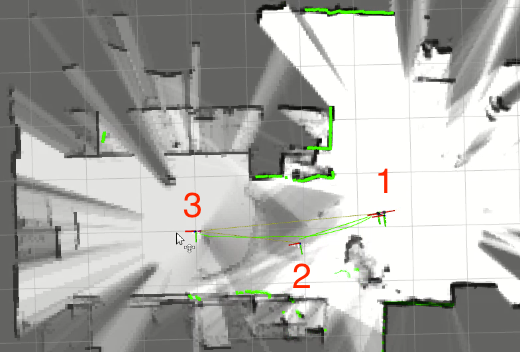
\includegraphics[width=0.97\textwidth]{./imgs/dynamic_objects/an_frame_1.png}
        \caption{Frame 1: Generated trajectory to goal}
        \label{fig:avoid_obs_1}
    \end{subfigure}%
    \begin{subfigure}{0.5\textwidth}
        \centering
        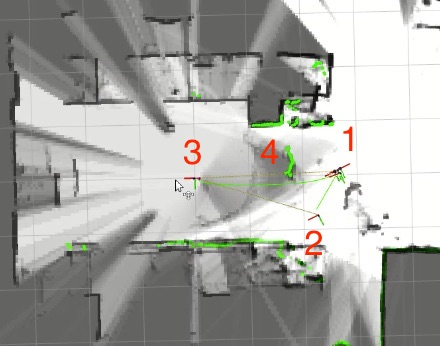
\includegraphics[width=0.97\textwidth]{./imgs/dynamic_objects/an_frame_2.png}
        \caption{Frame 2: Re-generated trajectory to goal to avoid obstacle}
        \label{fig:avoid_obs_2}
    \end{subfigure}
    \caption{Experiment conducted showing drone avoiding dynamic obstacles.  (1) Drone location (2) Local trajectory goal (3) Global goal (4) Dynamic obstacle\label{fig:avoid_obs}}
\end{figure}

Figure \ref{fig:avoid_obs_1} shows the first stage of the experiment where the drone was asked to generate a trajectory from it's current position to the global goal.  During it's progression along the trajectory an obstacle obstructed it's path.   Figure \ref{fig:avoid_obs_2} shows that a new local trajectory goal was able to be generated to give suitable clearance from the obstacle.  The drone was able to reach the original goal setpoint.\\

From this experiment we conclude that the drone is able to avoid dynamic obstacles in a laboratory setting.  However further testing could still be carried out.  A large gap between the drone and obstacle (1 metre) gave time for the drone to respond.  In subsequent tests this gap should be reduced to find the limitations of the obstacle avoidance capability.

\subsection{Turning Corners}
To be able to navigate an environment one core capability required is to be able to turn corners.  Demonstrating ability to turn corners also illustrates the drones capability to navigate into previously unseen environments and avoid static obstacles.

To evaluate the ability of the drone to turn corners the following experiment was conducted:
\begin{enumerate}
    \item place goal setpoint at an unseen location around a corner
    \item record any collisions 
\end{enumerate}
Success was measured if the drone was able to navigate to the goal setpoint without any collisions.
This experiment resulted in a number of changes to the trajectory generator and cost functions to meet the criteria.



\begin{figure}[H]
    \centering
    \begin{subfigure}{0.5\textwidth}
        \centering
        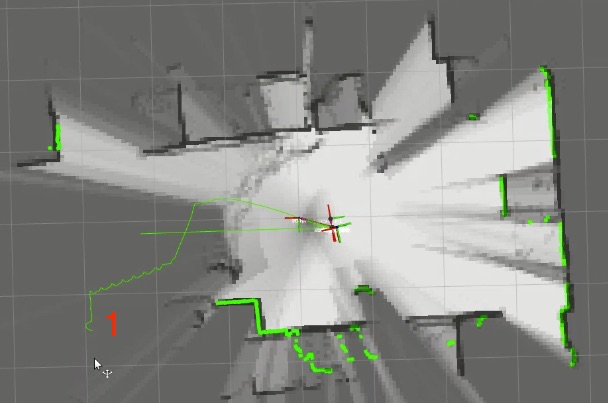
\includegraphics[width=0.97\textwidth]{./imgs/turn_corners/an_frame_1.jpg}
        \caption{Frame 1: Global setpoint placed in unseen environment around corner}
        \label{fig:avoid_obs_1}
    \end{subfigure}%
    \begin{subfigure}{0.5\textwidth}
        \centering
        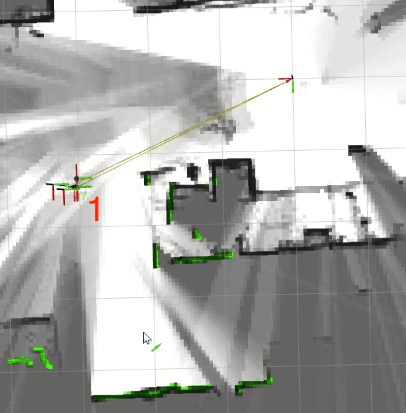
\includegraphics[width=0.97\textwidth]{./imgs/turn_corners/an_frame_2.jpg}
        \caption{Frame 2: Drone reached global setpoint}
        \label{fig:avoid_obs_2}
    \end{subfigure}
    \caption{Experiment showing drone turning corners (1) Global setpoint\label{fig:avoid_obs}}
\end{figure}

\subsection{Narrow Passageways}

\section{Future roadmap and limitations}
In this section, potential future additions to the drone and limitations of the present prototype will be discussed.  It makes sense to discuss these items together, since many of the items on the future roadmap arise by being limitations of the current prototype. In many cases, these limitations are by design and are an artifact of the team intentionally restricting an otherwise open-ended scope. \\

As outlined in the scope, the UAV prototype is limited to use in an indoor environment, with no considerations for dynamic variables. For our UAV to be able to meet the long-term goals of the MFB and operate in real-life disaster scenarios, the following features must be explored:
\begin{itemize}
\item 3D-Mapping: Due to limitations in processing power and bitrate of the communication link, it was decided that 2D mapping was most appropriate for our project (see Hardware selection and Drone selection ), leading to the use of a single Hokuyo URG-04LX-UG01 LIDAR scanner, capable of taking 2D ‘cross-sections’ of a 3D model by operating at different set altitudes. Fundamentally, less information is captured, with obstacles that cover a small range of altitudes potentially avoiding capture by the LIDAR scanner altogether resulting in less accurate information about the environment. For the drone to understand its surroundings fully, means of modelling its surroundings as a 3D space is required.  \\

Obtaining and using a more powerful processor and/or a higher capacity communication channel to a terrestrial base station; a relatively minor task, a simple solution is to use a 3D scanner, to generate a dense point cloud that represents the environment. These point clouds may be directly analysed and rendered as an environment layout, or converted to mesh models to increase object coherence and the usefulness of the outputted data. \\

This can also be achieved in the visual domain, using the Erlecopter’s onboard camera or another passive visual camera to simulate Structure from Motion (SfM) photogrammetric techniques. By moving through an environment (whilst periodically taking photos), and having navigation algorithms centred on directing the UAV along the detected boundaries of the environment, facing towards the centre where possible, local features in the environment can be detected. Commonly, the Difference of Gaussian (DoG) algorithm is used to help identify features, discarding a large range of spatial frequencies in an image, preserving only the spatial information that represent the edges of a feature. Random Sample Consensus (RANSAC) algorithm is then applied to remove incorrectly matched features, by iteratively estimating a mathematical model for the dataset produced and removing outliers. Based on memory and processing power available, this SfM method can be carried out globally; where the constituent samples of an environment are reconstructed at the same time or incrementally; solving image correspondence on a sample-to-sample basis. Realistically, an out-of-core solution is required as an intermediate approach, to combine partial reconstructions of sub-environments (e.g. rooms) due to wide range of environments that the UAV will operate in.\\

Many software solutions that package Patched-Based Multi-View Stereo (PVMS) and Clustering Views for Multi-view Stereo (CMVS) exist and can be integrated into UAV software, to save time.
\item Resistance to weathering and heat: As disaster management UAVs should be able to reach places that humans can’t, future UAV developments based off our prototype should be robust against any environment. For MFB purposes, such a UAV should be flame retardant and fireproof. An aluminium frame structure is recommended for its high melting point and light weight. However, despite its comparatively larger specific heat capacity
\item Multi-UAV systems: To enhance efficiency of the mapping process and reduce some of the fundamental limitations that are present in our prototype, namely processing power, many UAVs, behaving as nodes can be used. Multi-hop communication to cover disaster-affected areas may prove  can communicate rapidly to cover a greater area.
\end{itemize}

\section{Conclusion}
In this report, we have presented the core elements of a system which allows indoor autonomous navigation of an unmanned aerial vehicle. Live vision is provided to a base station, and the system is suitable for deployment in hazardous environments which may be unsafe for humans. We have delivered on the majority of our scope to MFB, and have demonstrated the feasiblity of this novel approach to disaster management.

\end{document}